\section{Data Collection and Graph Generation}

Every time a latency test completes—this is a test designed to evaluate the impact 
of delay on the prototype's performance—the testing mechanism contacts the logger 
via the /stat endpoint. The test data collected is then written into a JSON file:
  
\begin{listing}[H]
  \begin{minted}{json}
[
  {
    "delay_time": "0.0",
    "latency": 0.04399871826171875
  },
  ...
]
  \end{minted}
  \caption{Latency data obtain from the logger}
  \label{code:latency_json}
\end{listing}

The resulting JSON file follows the naming convention: algorithm\_name\_\%Y-\%m-\%d\_\%H-\%M-\%S.json. As an example, a file could be named as maekawa\_2023-06-07\_09-21-36.json, where 'maekawa' is the name of the algorithm being tested, and the rest of the filename corresponds to the timestamp (date and time) when the file was first created.

Utilizing the value of \textit{delay\_time} as the x-axis and \textit{latency} 
as the y-axis from the data outlined in \ref{code:latency_json}, tools such as 
numpy and matplotlib enable us to create illustrative graphs. These visualizations can provide a clearer understanding of the data:

\begin{figure}[H]
  \centering
  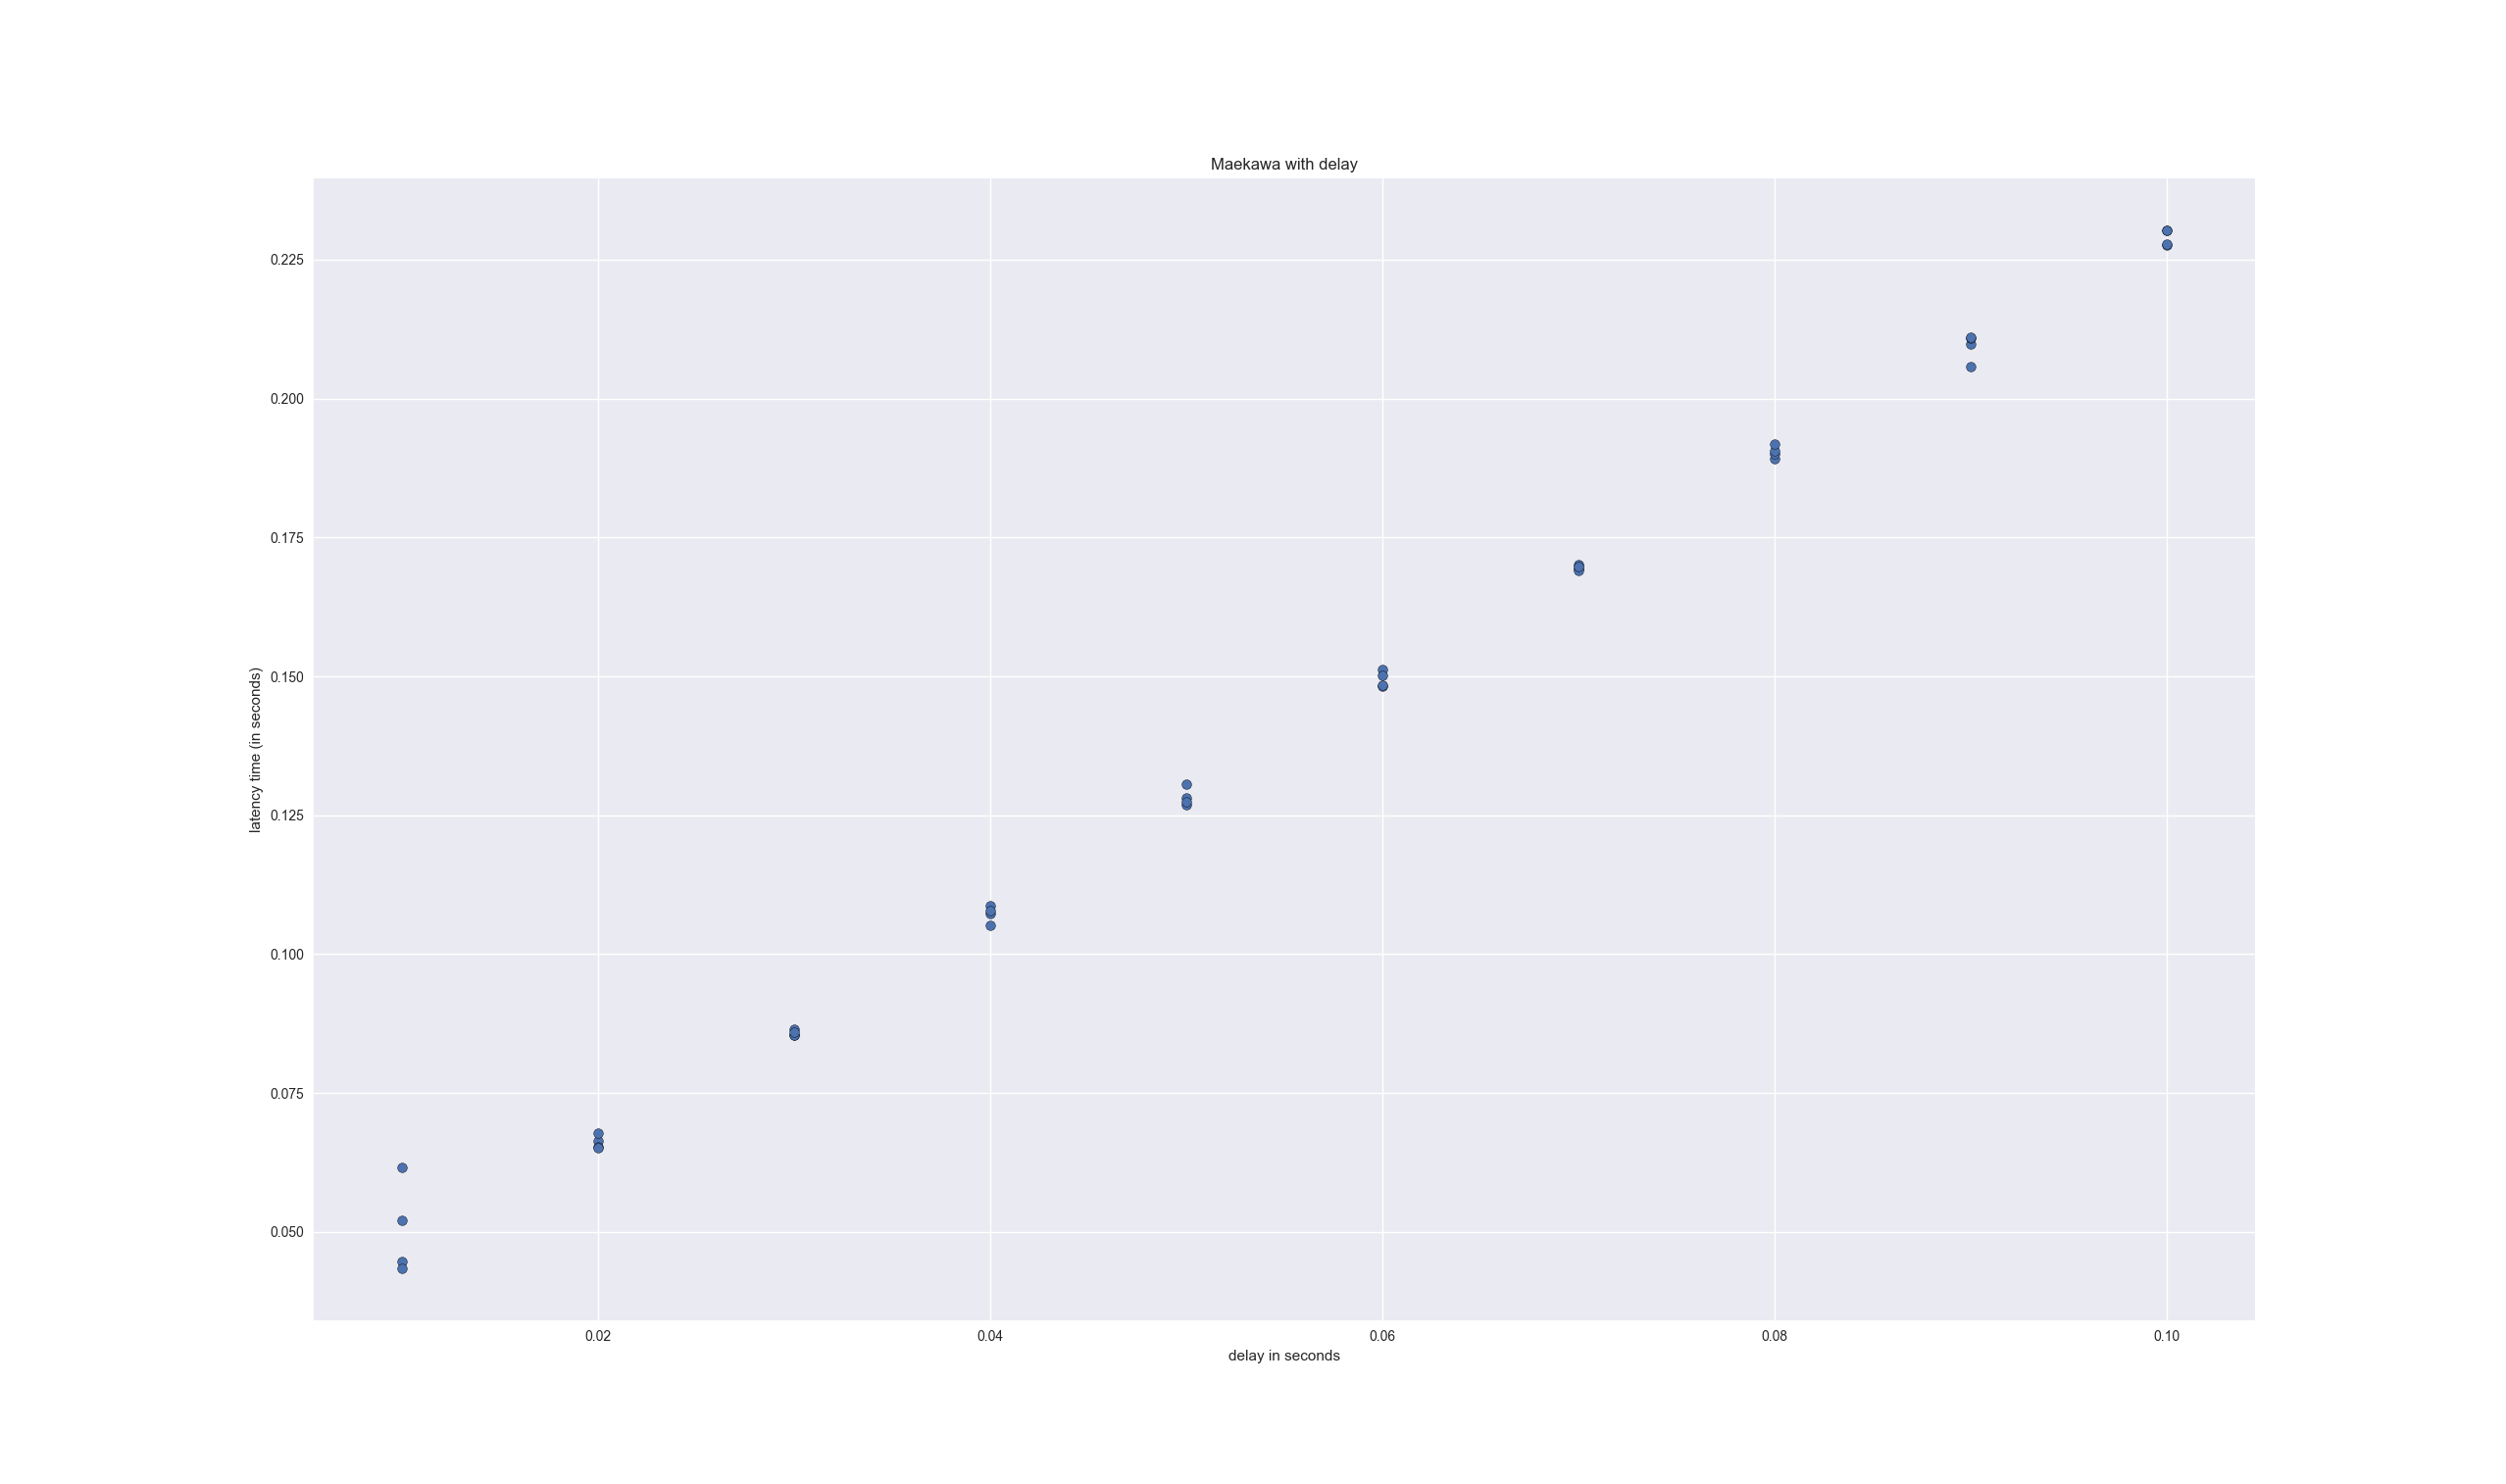
\includegraphics[width=\linewidth,height=\textheight,keepaspectratio]{maekawa_delay.png}
  \caption{Scatter plot between latency and delay in Maekawa algorithm}
\end{figure}

\begin{figure}[H]
  \centering
  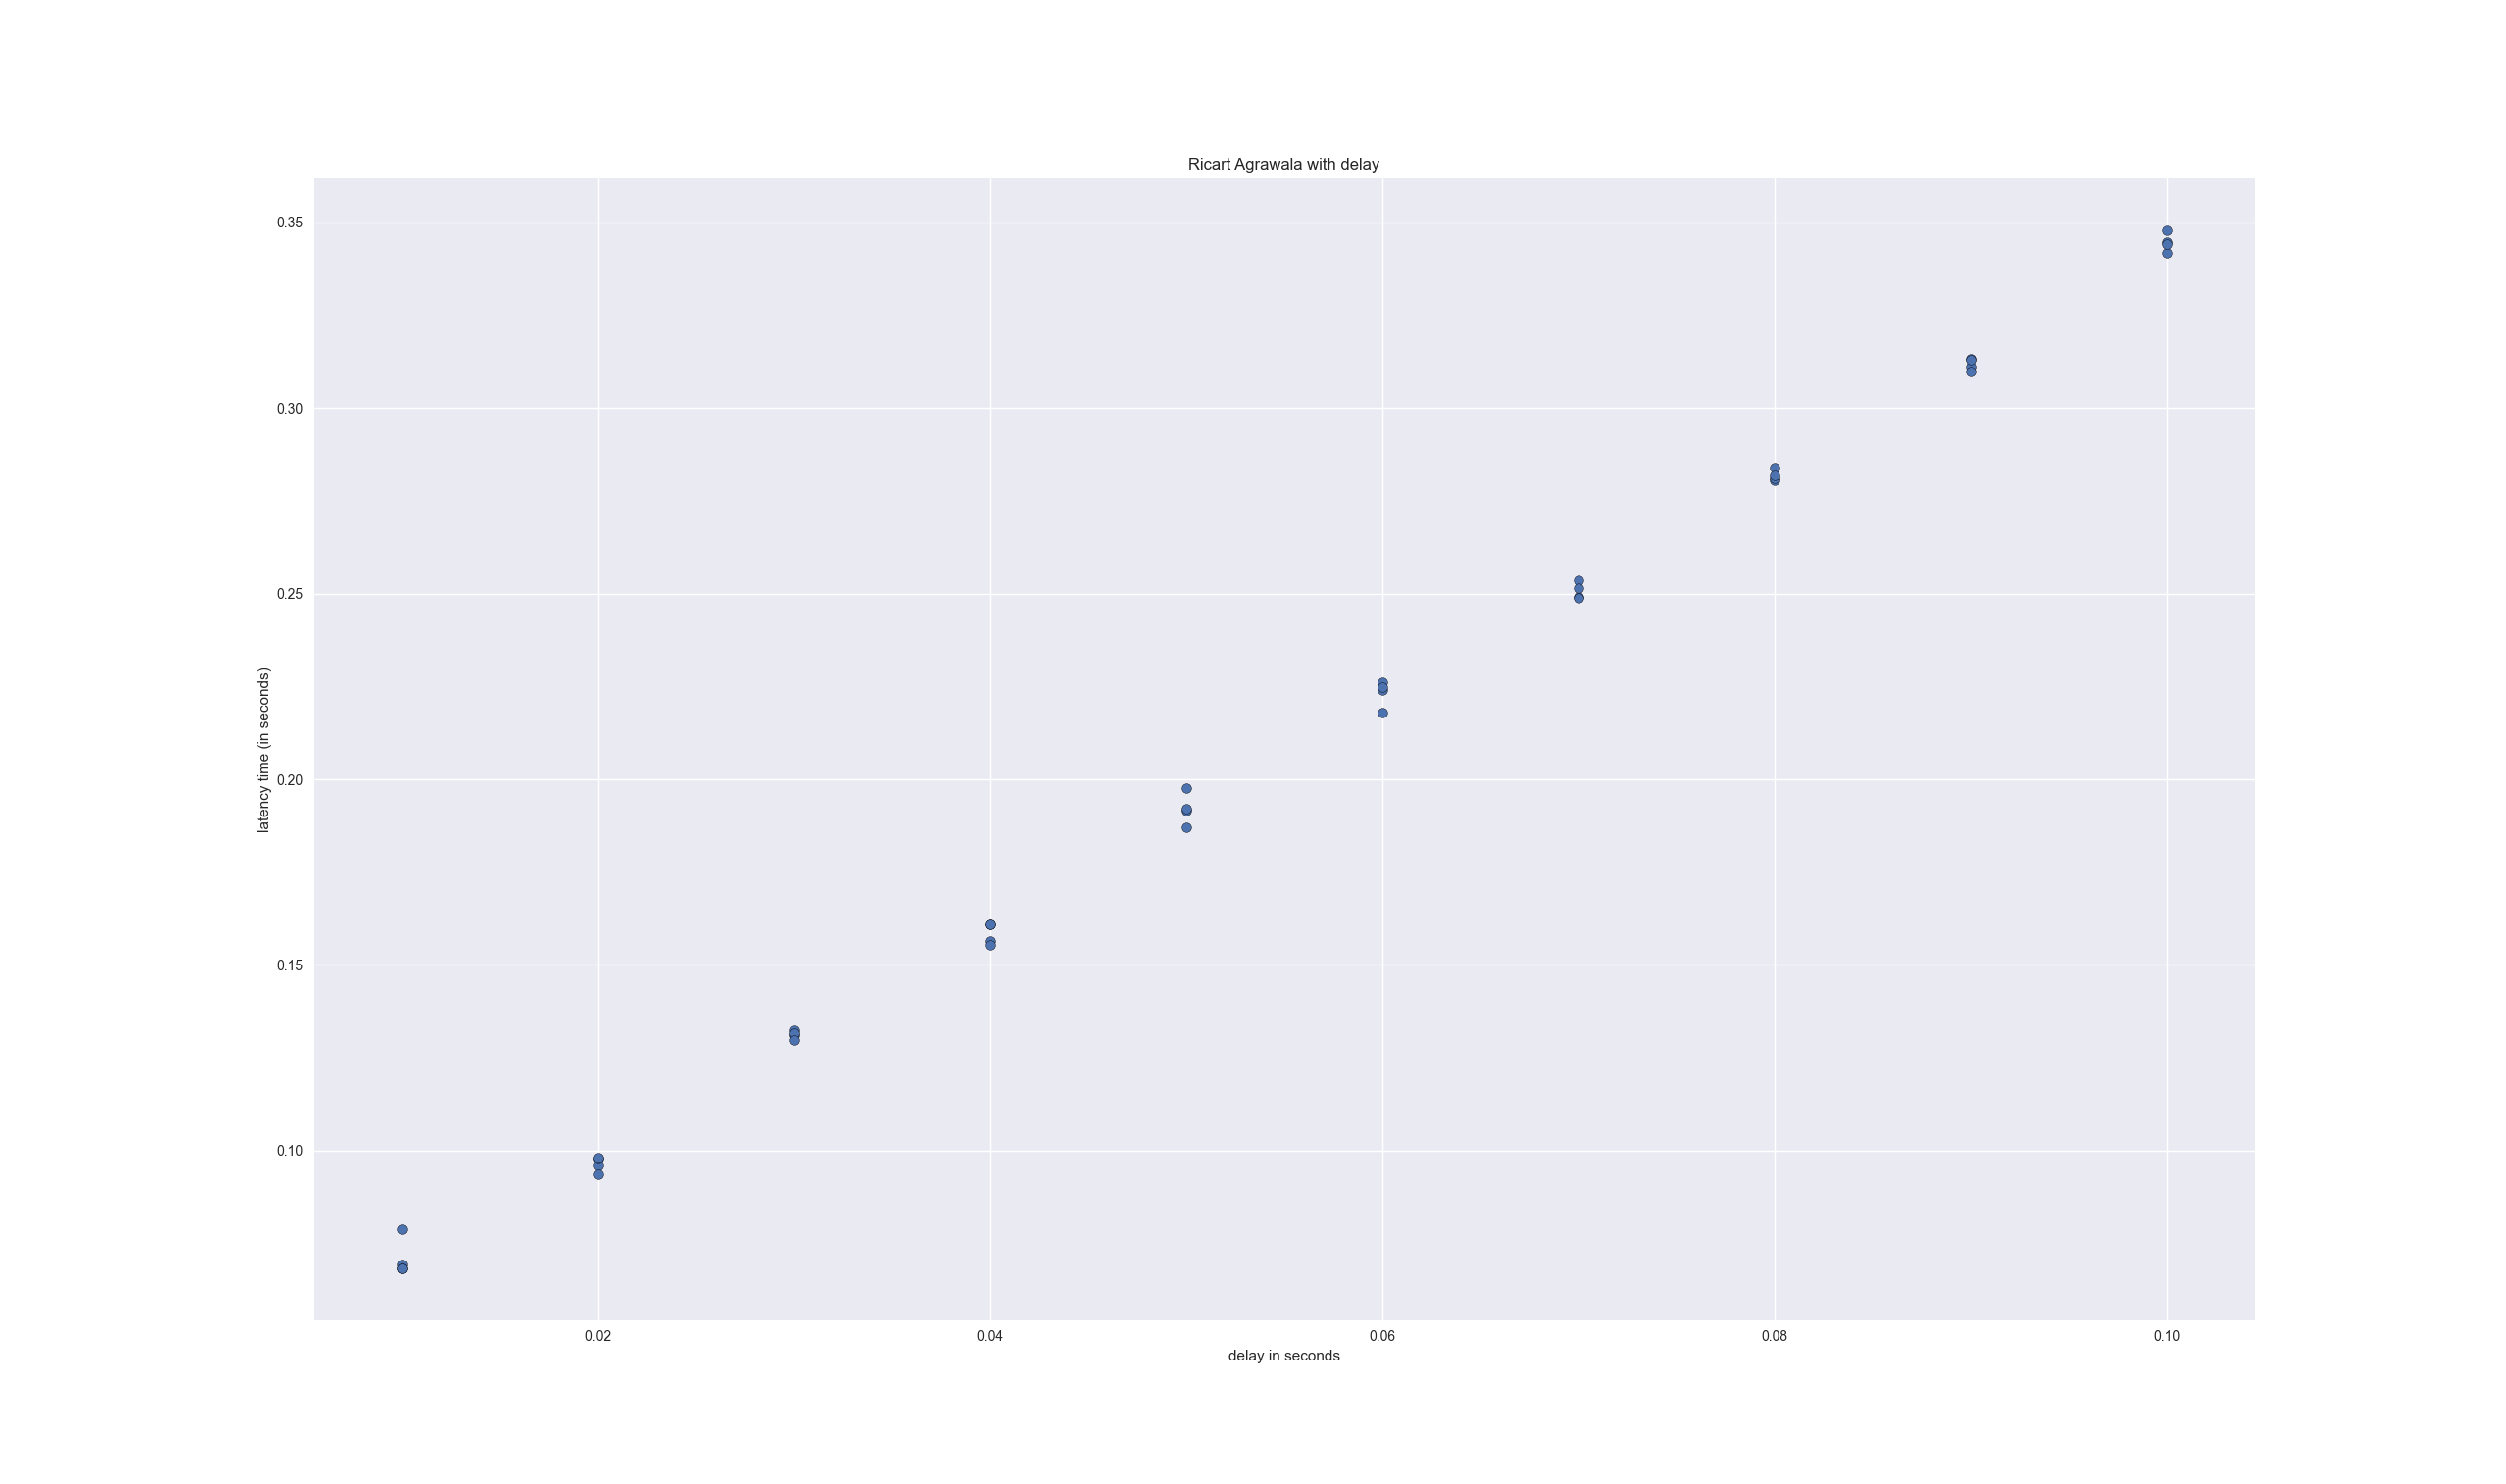
\includegraphics[width=\linewidth,height=\textheight,keepaspectratio]{ricart_agrwala_delay.png}
  \caption{Scatter plot between latency and delay in Ricart-Agrawala algorithm}
\end{figure}

Due to time constraints during the three-month internship phase, we were unable 
to conduct further exploration with error type fault and perform more extensive statistical tests.
